%
%
%
\subsection{Turbine cascade}
\label{stand11.subsec}
%
%
\begin{figure}
 \centerline{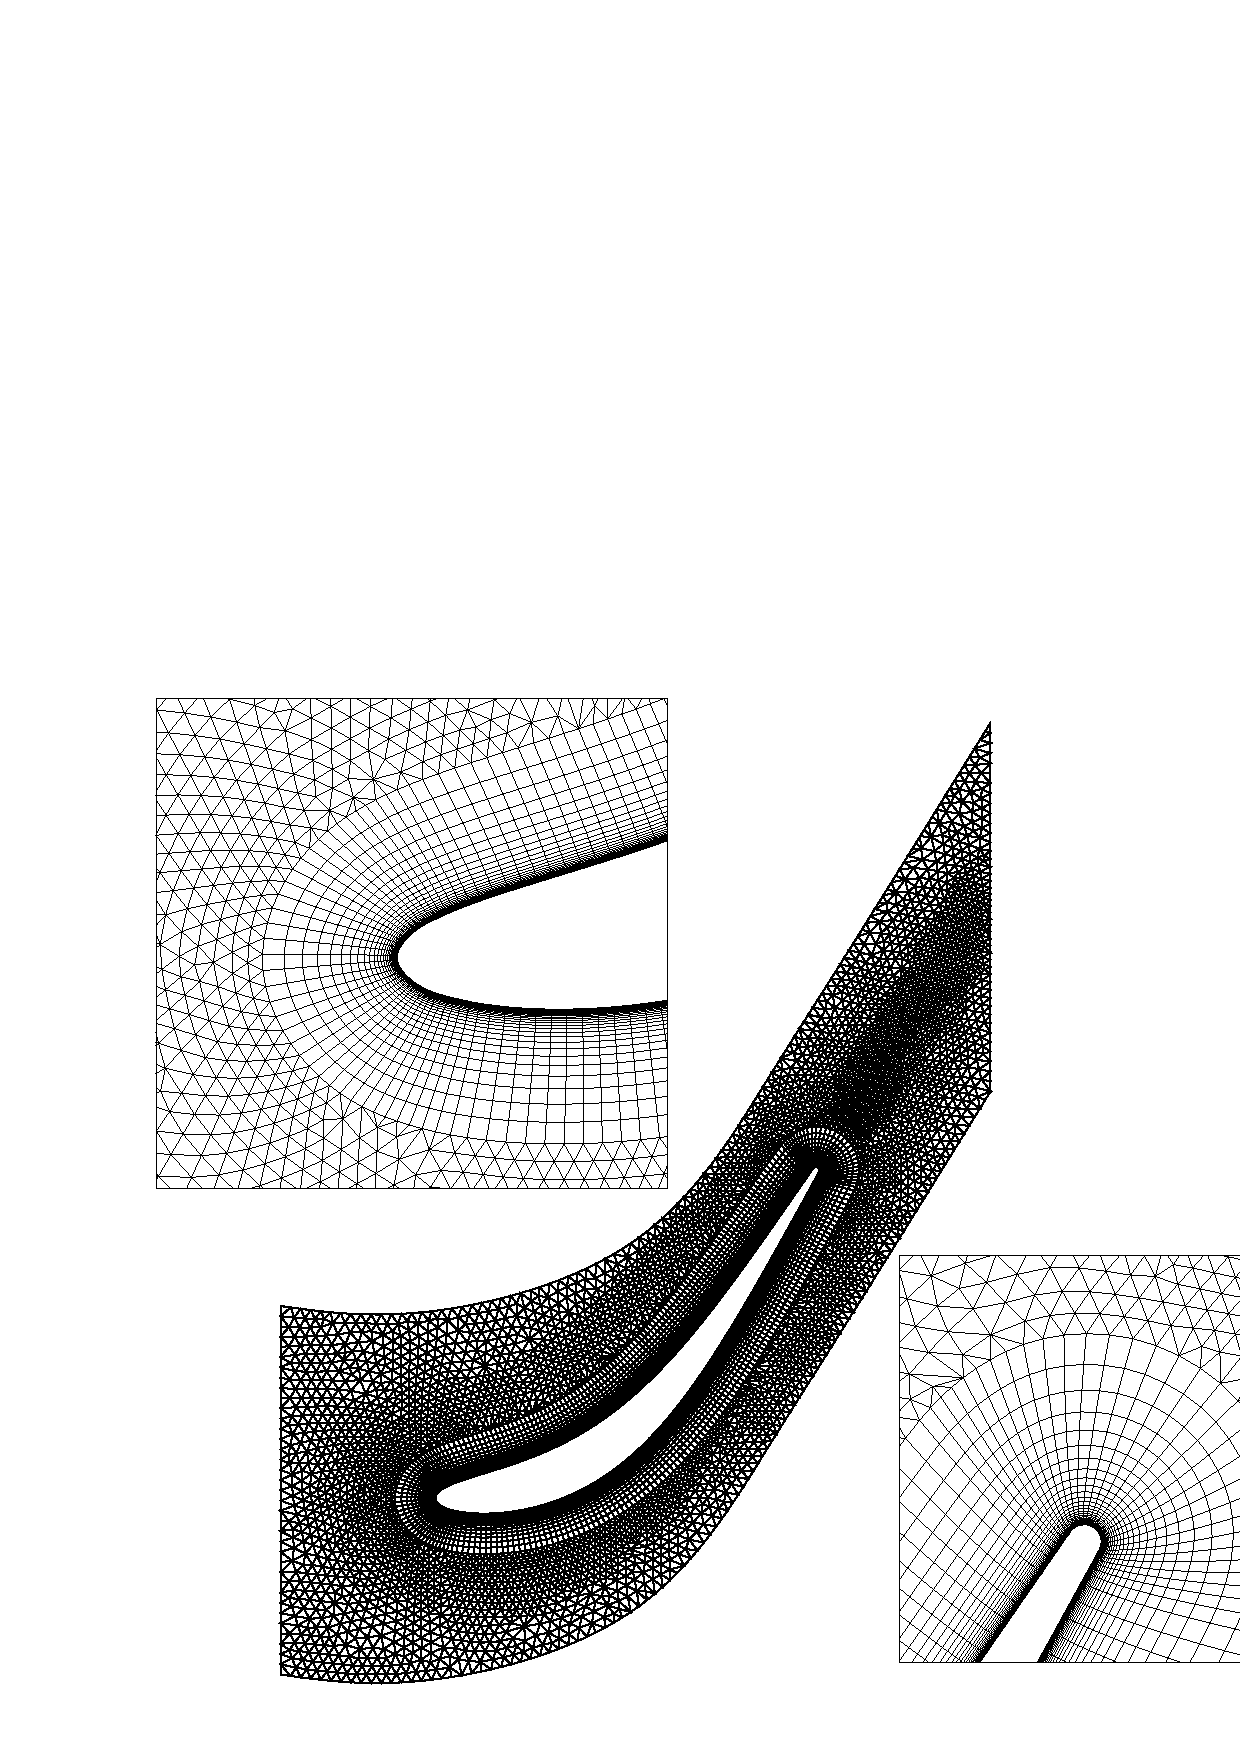
\includegraphics[width=120mm,clip=t]{CHAP_LINEAR/FIGURE/mesh_11th.pdf}}
 \caption{$11^{th}$ Standard configuration. Viscous mesh}
 \label{mesh_11th.fig}
\end{figure}
%
 In this Section the steady and unsteady flow due to bending motion
 of a turbine blade in the direction normal to its chord is analysed.
 The turbine blade geometry under consideration represents the
 $11\se{th}$ International Standard Configuration which have been
 studied for several flow regimes by Fransson et al.
 \citeyear{Bolcs:2}\footnote{The data for the International Standard Configurations
 can be found at {\bf http://www.egi.kth.se/ekv/stcf/} }.
 Two particular flows  will be considered here:
 a subsonic attached flow  and a transonic flow showing a separation
 bubble on the suction surface.
 Fig. \ref{mesh_11th.fig} shows the computational mesh used for all viscous
 calculations. There are 9,312 quadrilaterals in the
 boundary layer region and 7,751 triangles in the rest of the domain, the total  number
 of points being 13,481. A second mesh, used for the inviscid calculations, has
 been obtained from the viscous mesh of Fig. \ref{mesh_11th.fig} by simply removing
 the quadrilateral elements in the boundary layer.

\paragraph{Steady-state flow results.}
%
%
\begin{figure}
 \centerline{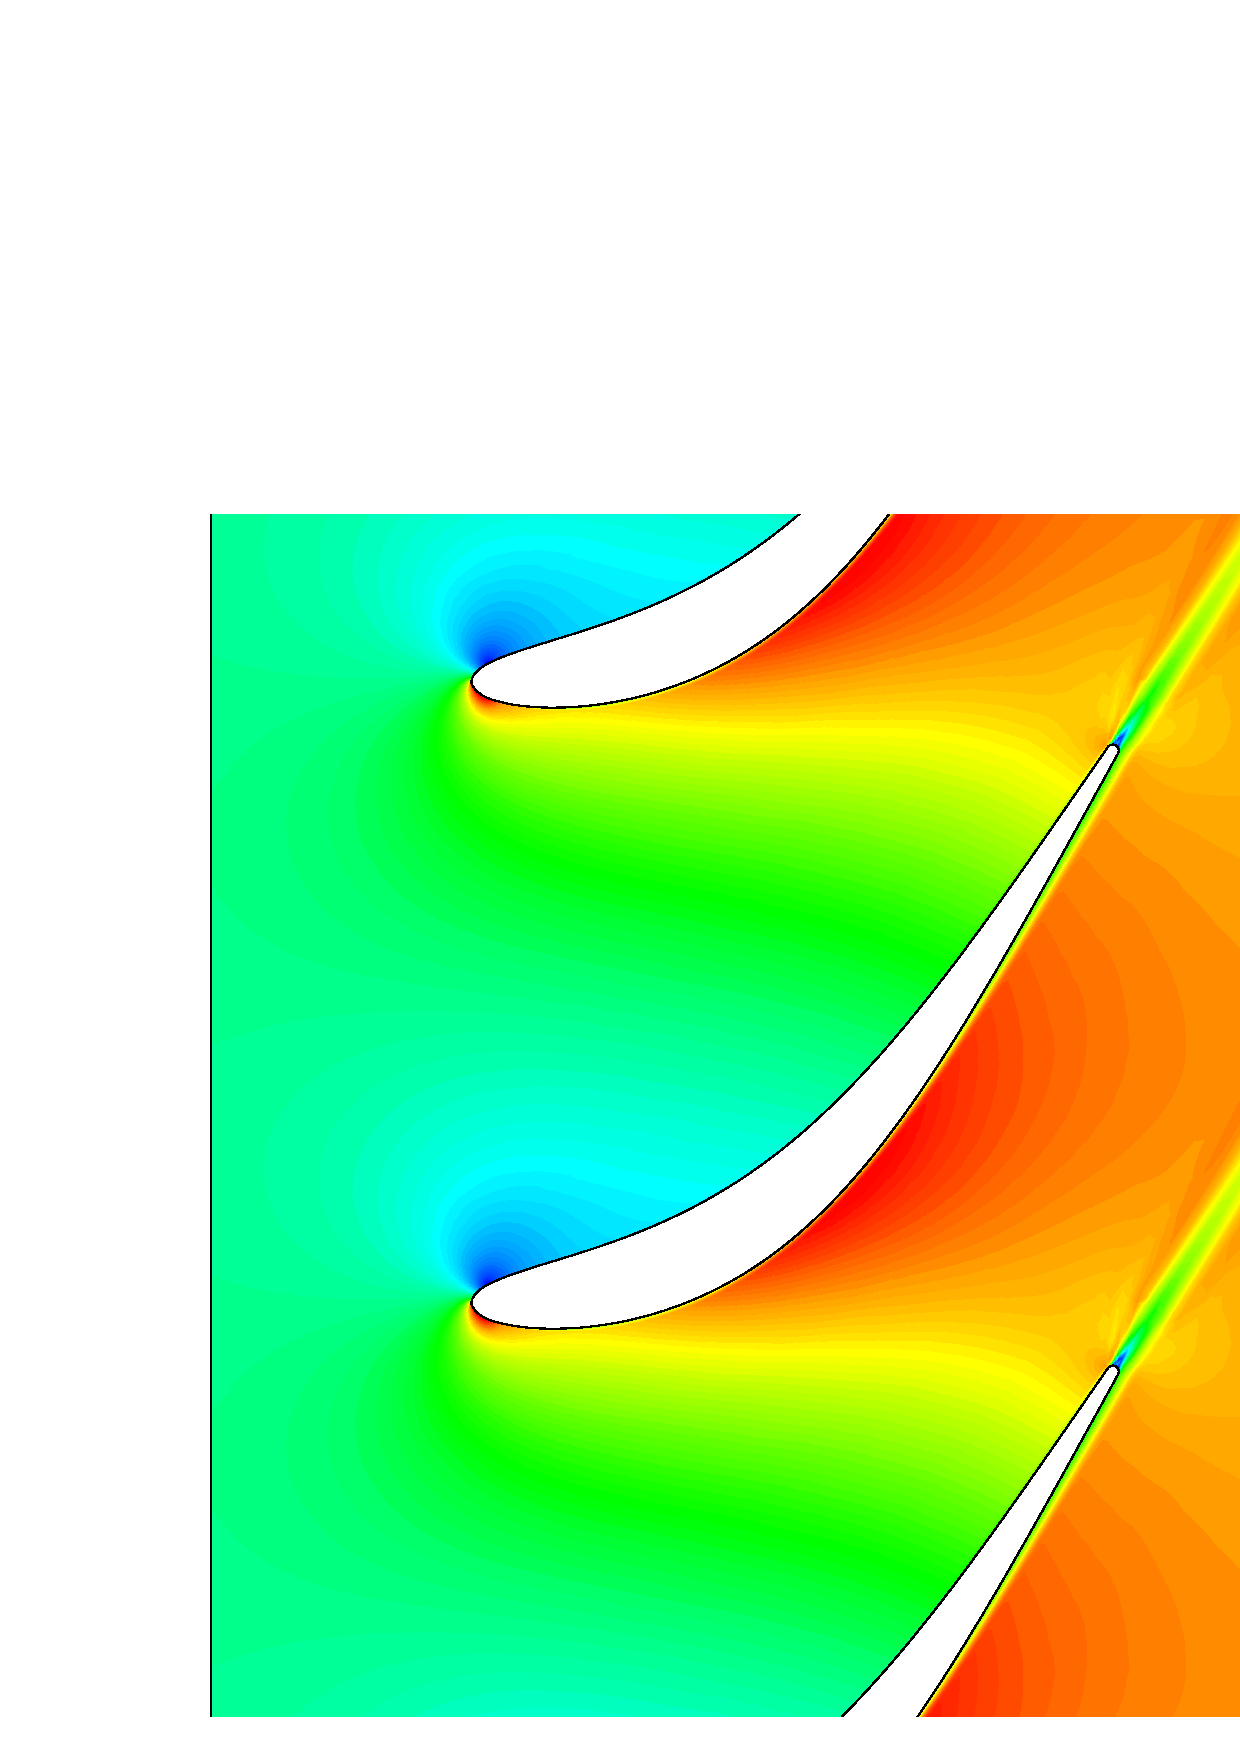
\includegraphics[width=100mm,clip=t]{CHAP_LINEAR/FIGURE/steady_11th_m069_mac_con.pdf}}
 \caption{$11^{th}$ Standard configuration - subsonic case. Steady-state Mach contours}
 \label{conf11_mac_con_069.fig}
\end{figure}
%
%
%
\begin{figure}[ht]
 \centerline{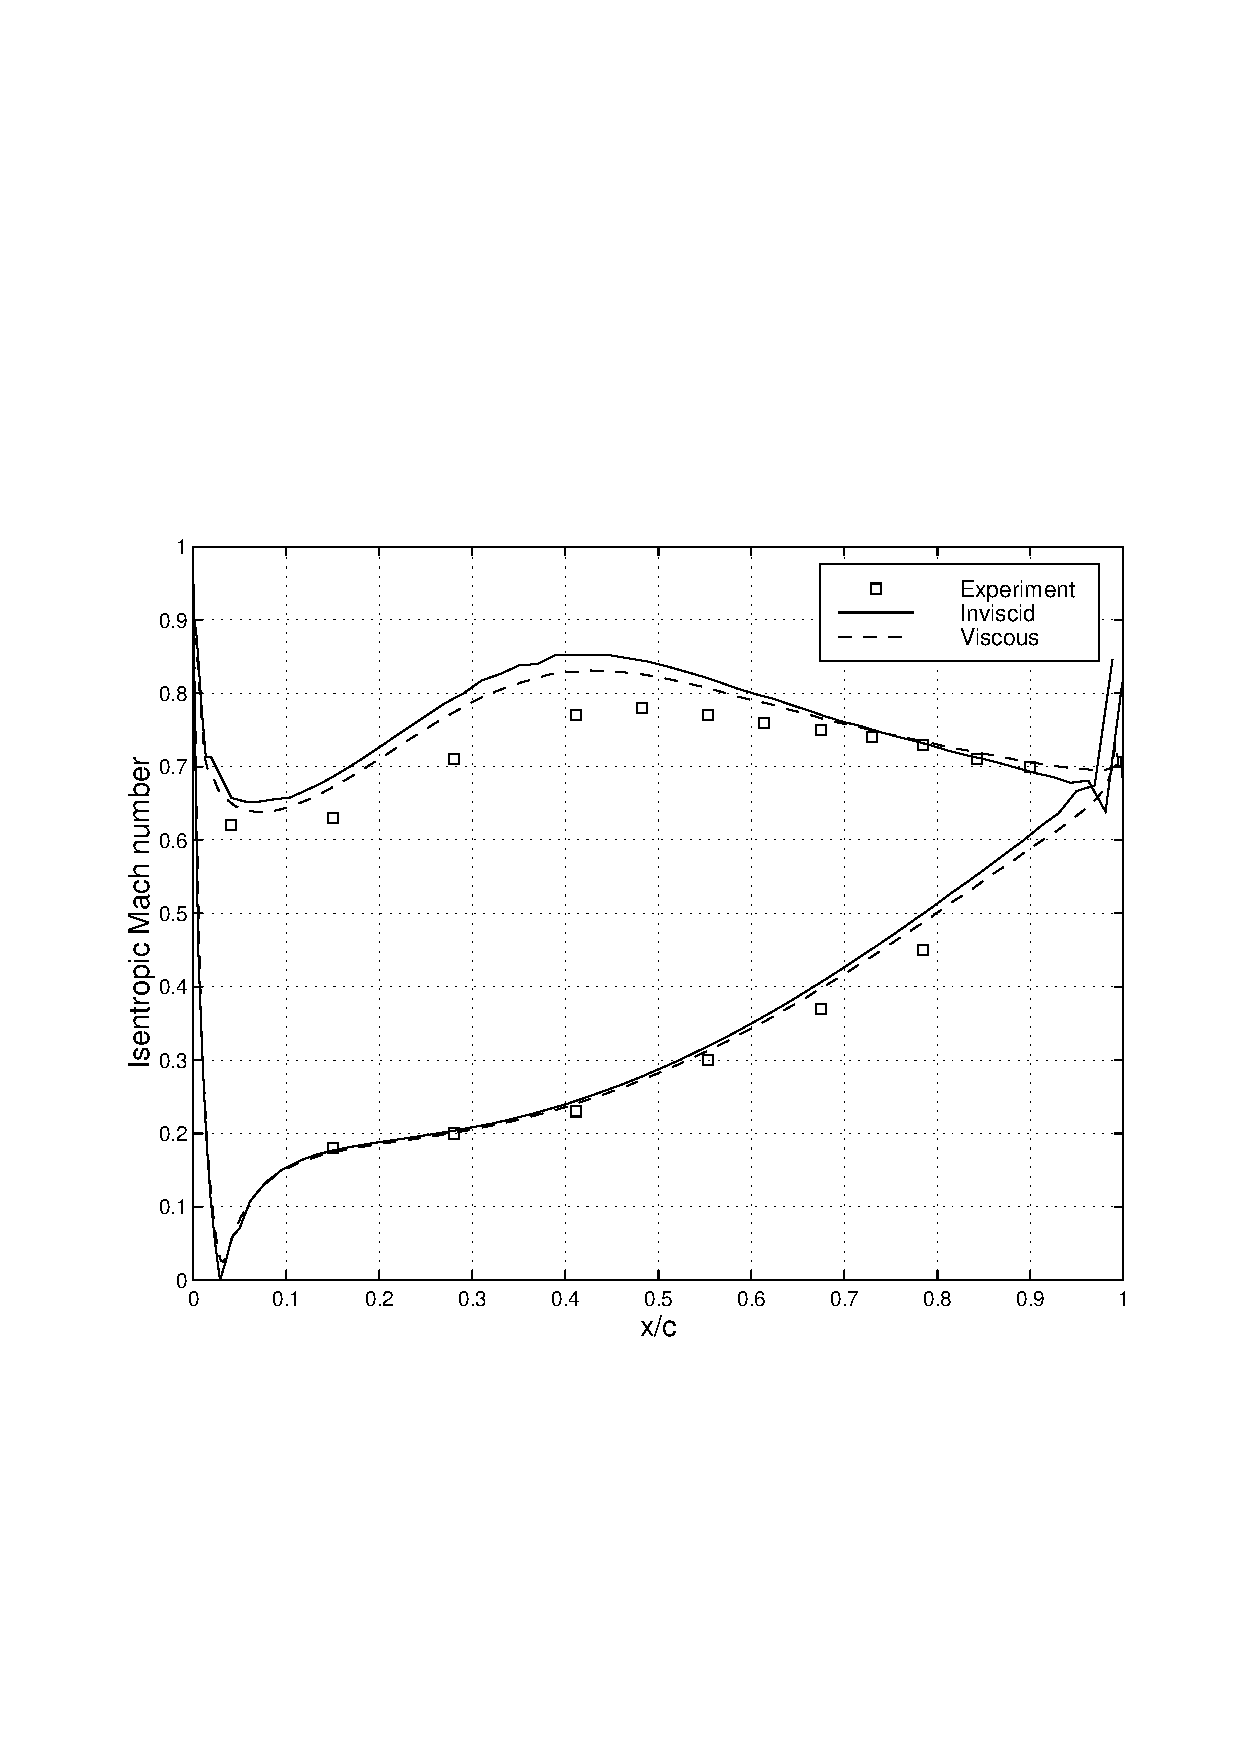
\includegraphics[width=130mm,clip=t]{CHAP_LINEAR/FIGURE/steady_11th_m069_mac_bla.pdf}}
 \caption{$11^{th}$ Standard configuration - subsonic case.
           Isentropic Mach number distribution on the blade}
 \label{conf11_mac_bla_069.fig}
\end{figure}
%
 For the subsonic flow case the inlet flow angle is $-15.2\se{o}$,
 the outlet isentropic Mach number is 0.69
 and the inlet Reynolds number, based on the blade's chord, is $650,000$.
 The maximum value of $y+$ is of around 4 which guarantees a good resolution of the
 viscous sublayer using the Spalart-Allmaras turbulence model.
 The predicted Mach number contours are shown in Fig. \ref{conf11_mac_con_069.fig}
 while a comparison of the inviscid and viscous analyses with measured data is given in
 Fig. \ref{conf11_mac_bla_069.fig}.
 For the suction surface, both the viscous and inviscid computations somewhat
 overpredict the Mach number distribution at around mid-chord. However, a similar
 solution was obtained by  Fransson et al. \citeyear{Bolcs:2} and the reasons for
 the discrepancy are discussed in some detail. Here, we will consider that the
 steady-state flow has been captured adequately for the purposes of providing a
 starting point for the linearised unsteady flow.

 For the transonic off-design case the inlet flow angle is $34\se{o}$,
 the outlet isentropic Mach number is $1$ and the inlet Reynolds number,
 based on the blade's chord, is $860,000$. The maximum $y+$ value is around 5.
 The predicted Mach number contours are plotted in Fig. \ref{conf11_mac_con_099.fig}a.
 A particular feature of the flow, the recirculation bubble on the suction
 surface, is shown in Fig. \ref{conf11_mac_con_099.fig}b.
 Because of the significant viscous features,
 the Navier-Stokes analysis shows a much better agreement
 with the measured data, with perhaps the exception of the trailing-edge behaviour
 (Fig. \ref{conf11_mac_bla_099.fig}).
 However, as discussed by Fransson et al. \citeyear{Bolcs:2}, the pre-shock
 Mach number is very sensitive to the experimental inlet conditions.
 In any case, as expected, a viscous
 analysis is required to predict  the separation bubble of the suction side which
 occurs between $10-30\%$  blade chord, a feature that can be seen from  the flow
 deceleration in Fig. \ref{conf11_mac_bla_099.fig}. As will be discussed below,
 such differences in the steady-state flow will lead to major
 discrepancies for unsteady flow predictions.
%
\begin{figure}[ht]
 \begin{center}
  \begin{tabular}{c}
    \subfigure[Mach contours]
       {\includegraphics[width=80mm,clip=t]{CHAP_LINEAR/FIGURE/steady_11th_m099_mac_con.pdf}}\\
    \subfigure[Particle traces in the separation bubble]
       {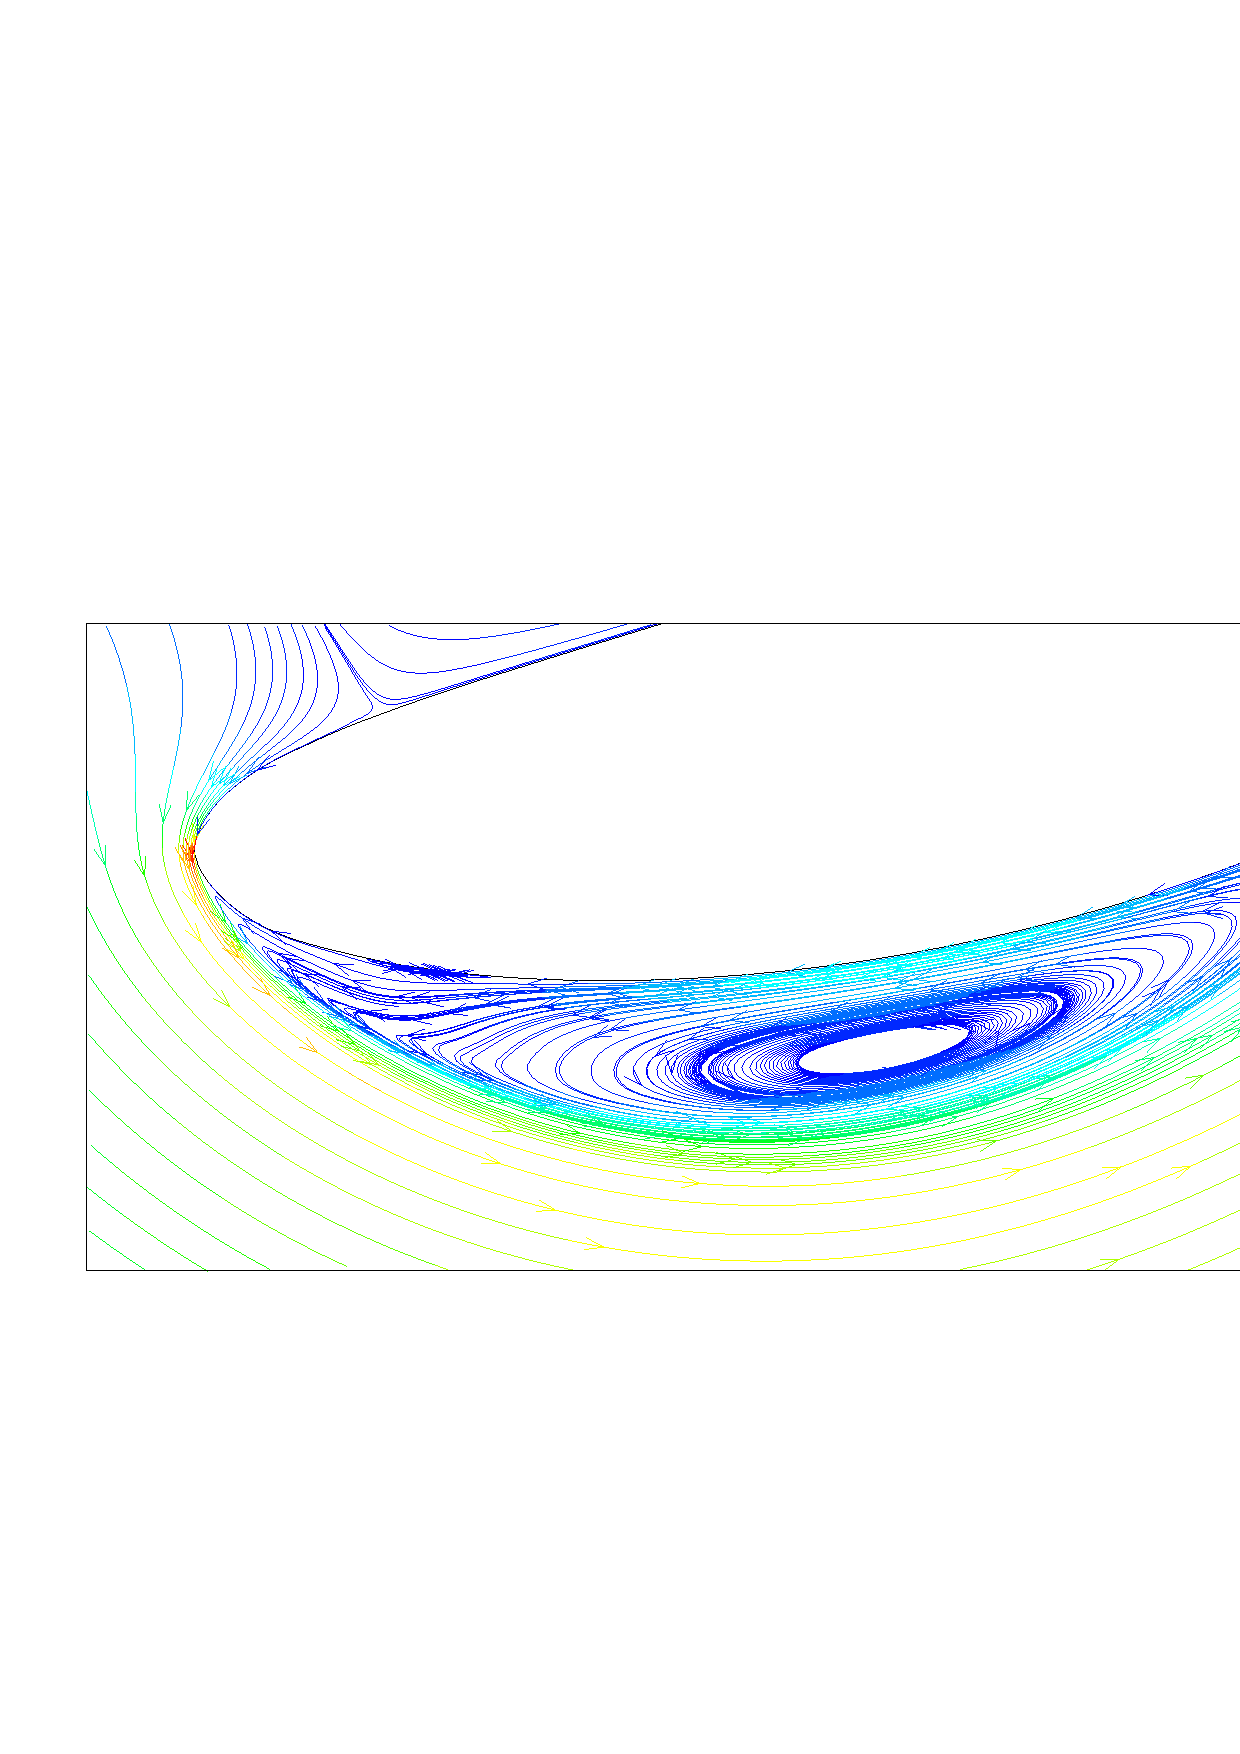
\includegraphics[width=80mm,clip=t]{CHAP_LINEAR/FIGURE/steady_11th_m099_stream.pdf}}
  \end{tabular}
 \end{center}
 \vspace{-7mm}
 \caption{$11^{th}$ Standard configuration - transonic case. Steady-state Mach contours}
 \label{conf11_mac_con_099.fig}
\end{figure}
%
%
\begin{figure}[ht]
 \centerline{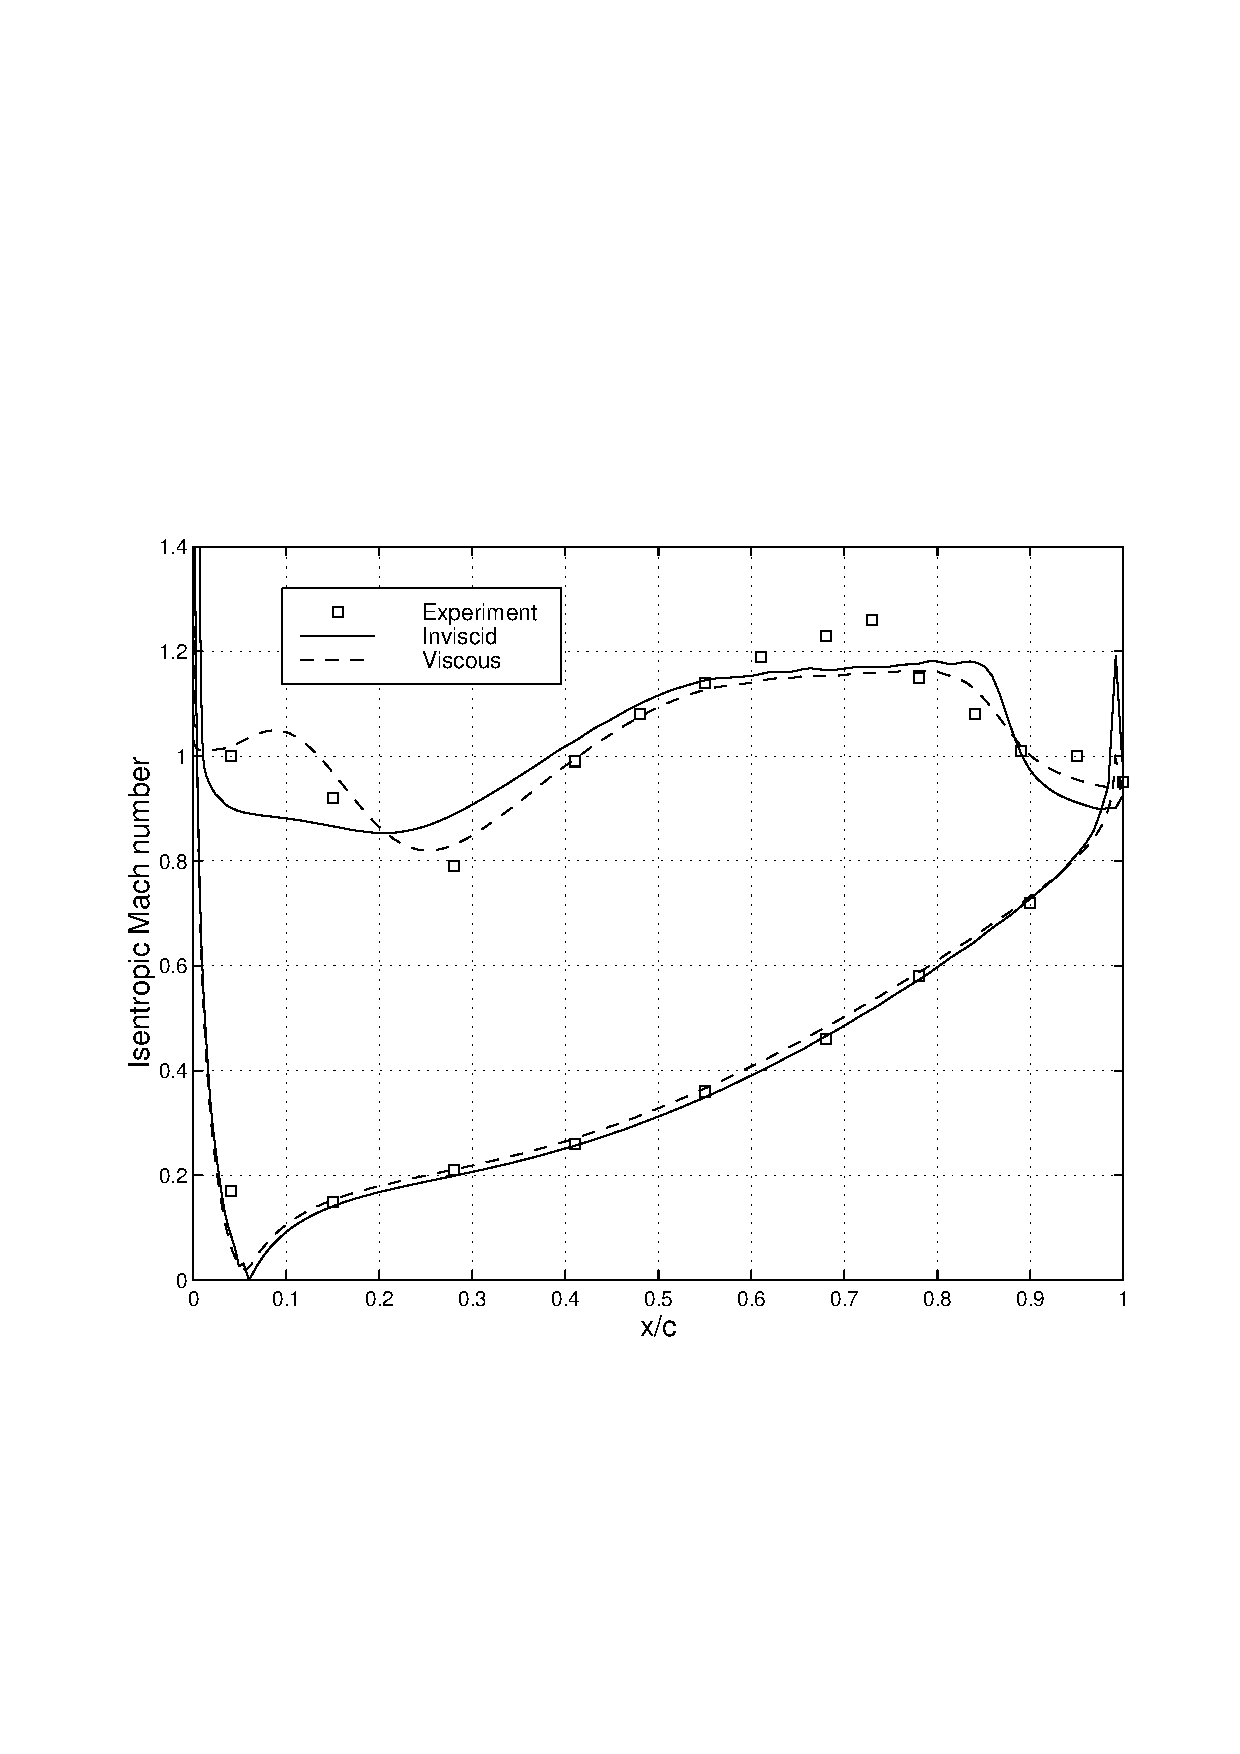
\includegraphics[width=130mm,clip=t]{CHAP_LINEAR/FIGURE/steady_11th_m099_mac_bla.pdf}}
 \caption{$11^{th}$ Standard configuration - transonic case.
           Isentropic Mach number distribution on the blade}
 \label{conf11_mac_bla_099.fig}
\end{figure}
%
%
%
\paragraph{Linearised unsteady flow results}
 The unsteadiness  due to bending motion
 of the blade in the direction normal to its chord was computed using the linearised
 flow solver. The  reduced frequency is 0.21 for the
 subsonic case and 0.15 for the transonic case.  Three different sets of flow calculations were
 performed for each case:  (i) inviscid linearised using an inviscid base steady-state flow,
 (ii) viscous linearised with frozen turbulence using viscous fully-turbulent
 base flow, and (iii) viscous fully-linearised  using the same viscous
 base flow as in (ii).
 In calculations (ii), neither the laminar nor the turbulent
 viscosities were linearised and their values were kept fixed at their steady-state values.
 Calculations (iii) were performed with a fully-linearised Spalart-Allmaras turbulence
 model.

 The amplitude and phase of the predicted unsteady
 pressure coefficient\footnote{$\widetilde{c}\sm{p} =
 \frac{c\, \widetilde{p}}{h\left(p\sm{01} - p\sm{1}\right)}$, where $h$ is the
 bending amplitude and $c$ the blade chord.}
 distribution are compared to measured data in Figs.
 \ref{subsonic_11_ampl.fig} and \ref{subsonic_11_phas.fig} for the subsonic case.
 The first noticeable feature is the similarity of the amplitude predictions for the
 three modelling levels, though some deviations can be observed for the phase plots.
 This result is somewhat expected because of the similarity of the inviscid and
 viscous steady-state solutions.
 There is reasonable overall agreement with the measured data, though the undershoot
 at around $50\%$ chord is not captured in any of the computations.
 An inspection of the phase plots reveals that the negative to positive
 (or stable to unstable)  phase jump, is predicted
 much further downstream than the measured position.
 However, the fully non-linear viscous unsteady calculations of Franson et al.
 \citeyear{Bolcs:2} exhibit the same trend and hence the cause of the discrepancy
 is not due to linearisation.

 The amplitude and phase of the predicted unsteady
 pressure distribution is compared to measured data
 in Figs. \ref{transonic_11_ampl.fig} and \ref{transonic_11_phas.fig}
 for the transonic case.
 The discrepancies between different the three modelling levels is now more pronounced.
 The linearised inviscid approach is seen to overpredict the unsteady
 pressure coefficient on the suction side of the blade both in the recirculation
 region ($0 - 30\%$ of chord) and around the trailing-edge.  In the recirculation region,
 the full linearisation of the viscous terms yields better results than freezing
 the turbulence model and the two approaches are seen to be equivalent elsewhere.
%
%
\begin{figure}
 \begin{center}
  \begin{tabular}{c}
    {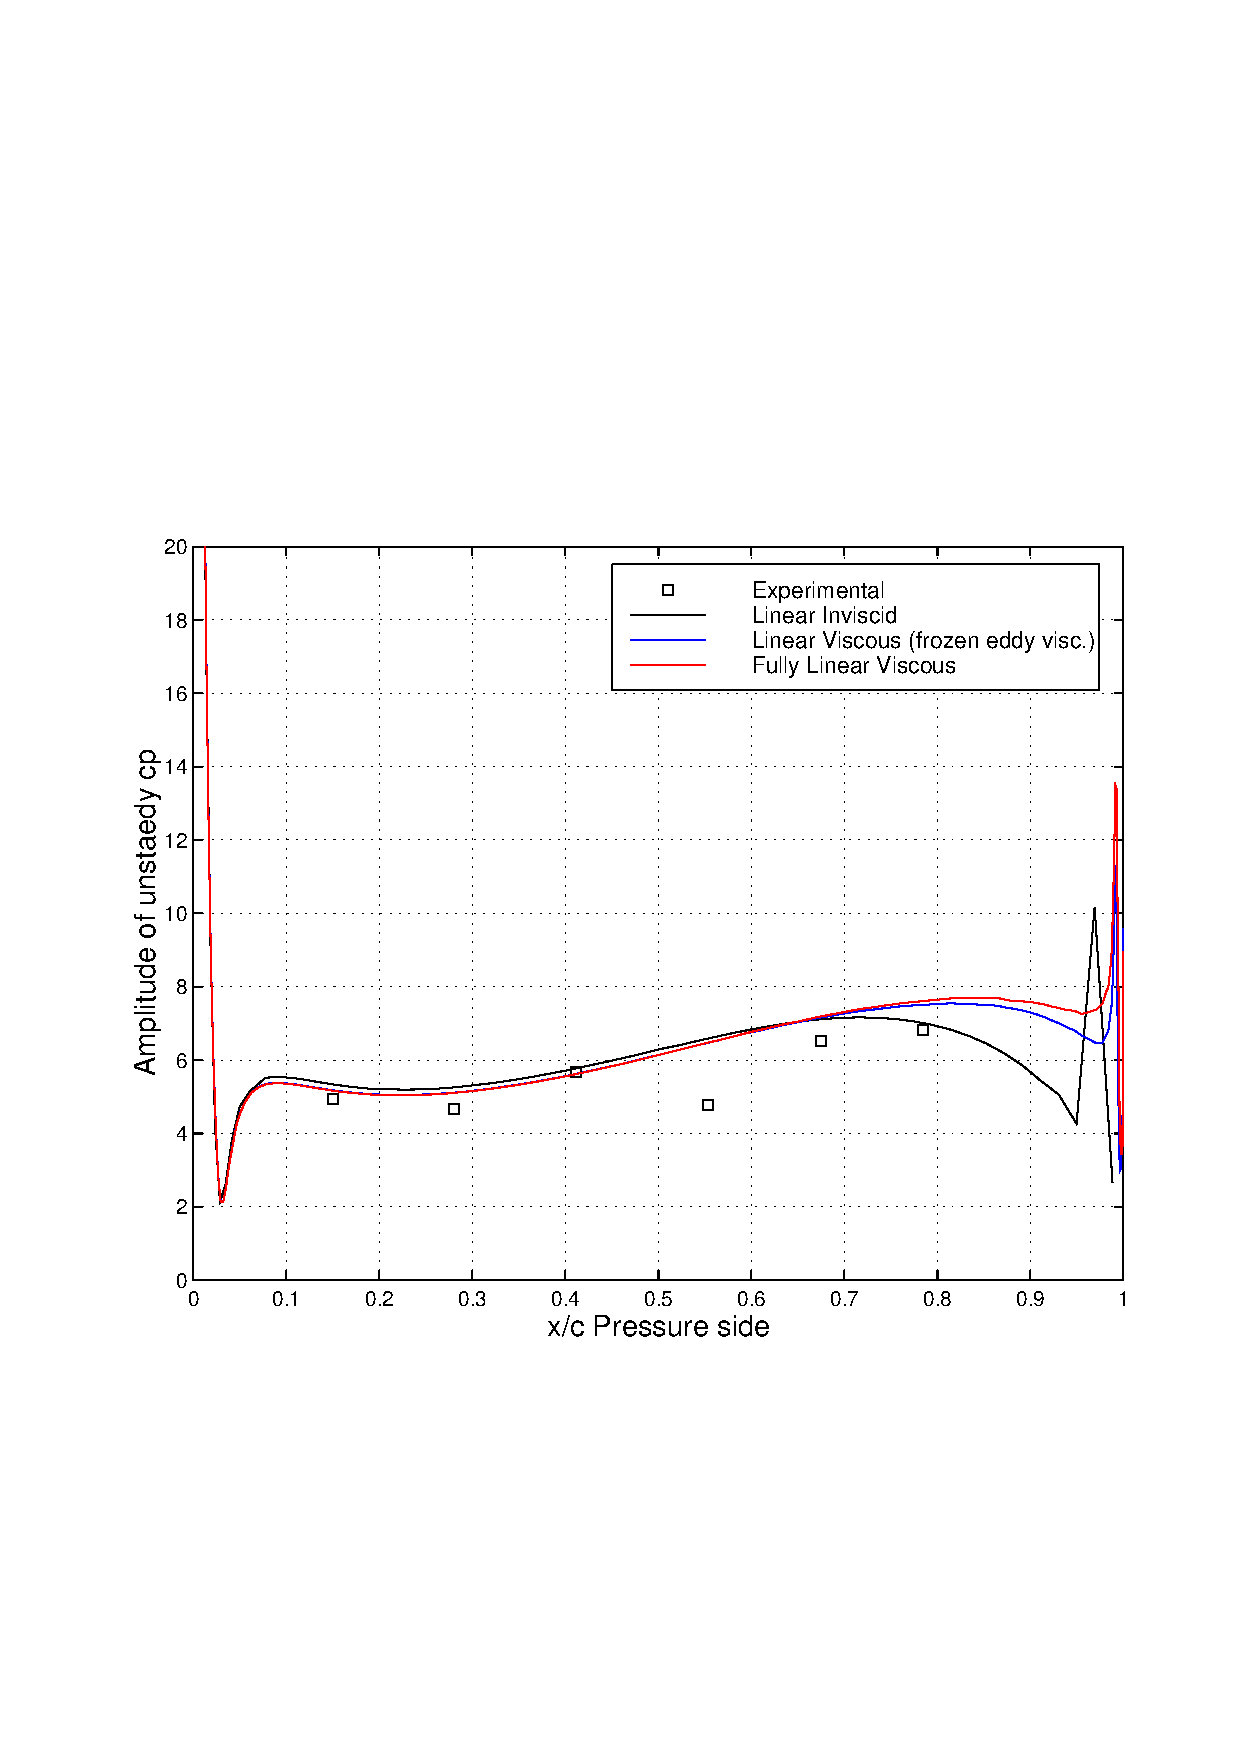
\includegraphics[height=100mm,clip=t]{CHAP_LINEAR/FIGURE/unsteady_blade_069_180_1.pdf}}\\
    {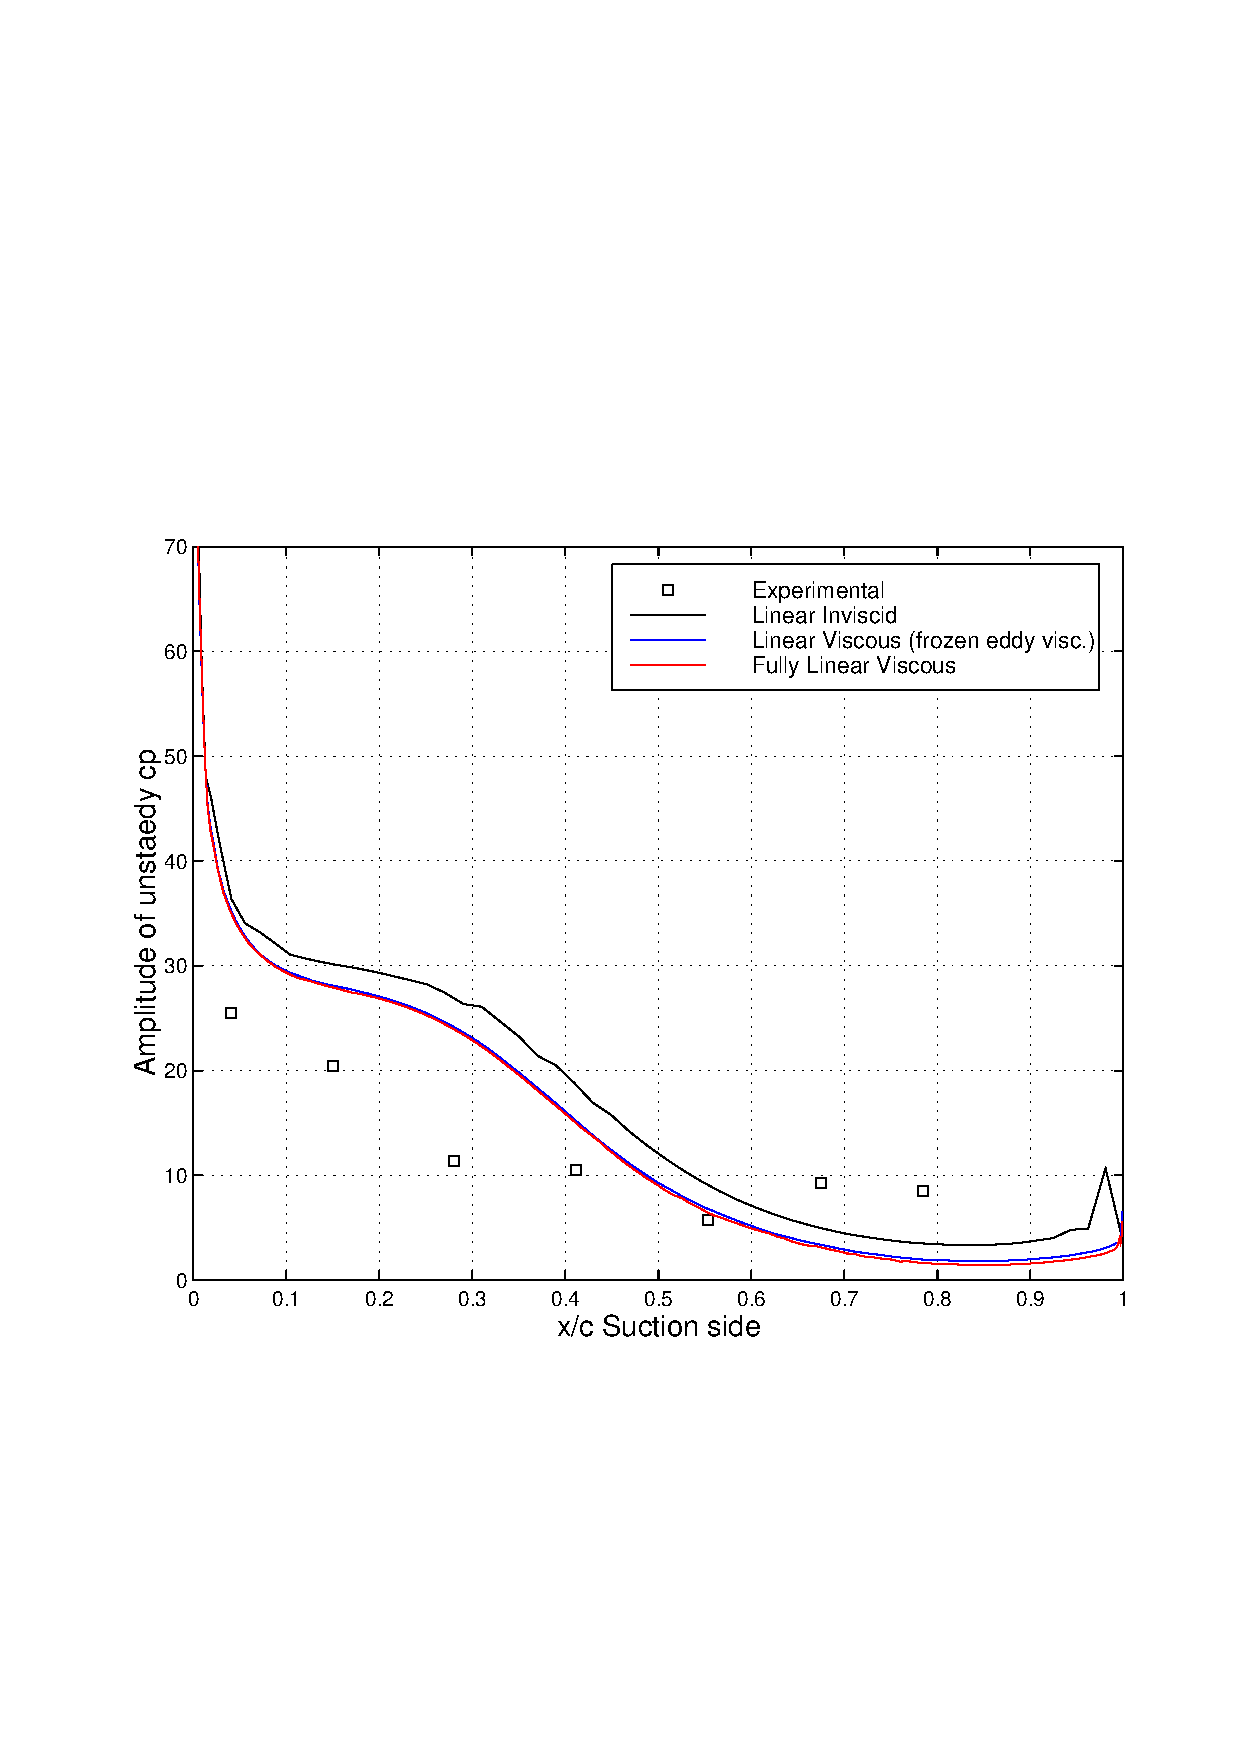
\includegraphics[height=100mm,clip=t]{CHAP_LINEAR/FIGURE/unsteady_blade_069_180_2.pdf}}
  \end{tabular}
 \end{center}
 \vspace{-7mm}
 \caption{$11^{th}$ Standard configuration - subsonic case.
          Amplitude of $\tilde{c}\sm{p}$
         ($\omega = 0.21$, $\phi = 180\se{o}$)}
 \label{subsonic_11_ampl.fig}
\end{figure}
%
\begin{figure}
 \begin{center}
  \begin{tabular}{c}
    {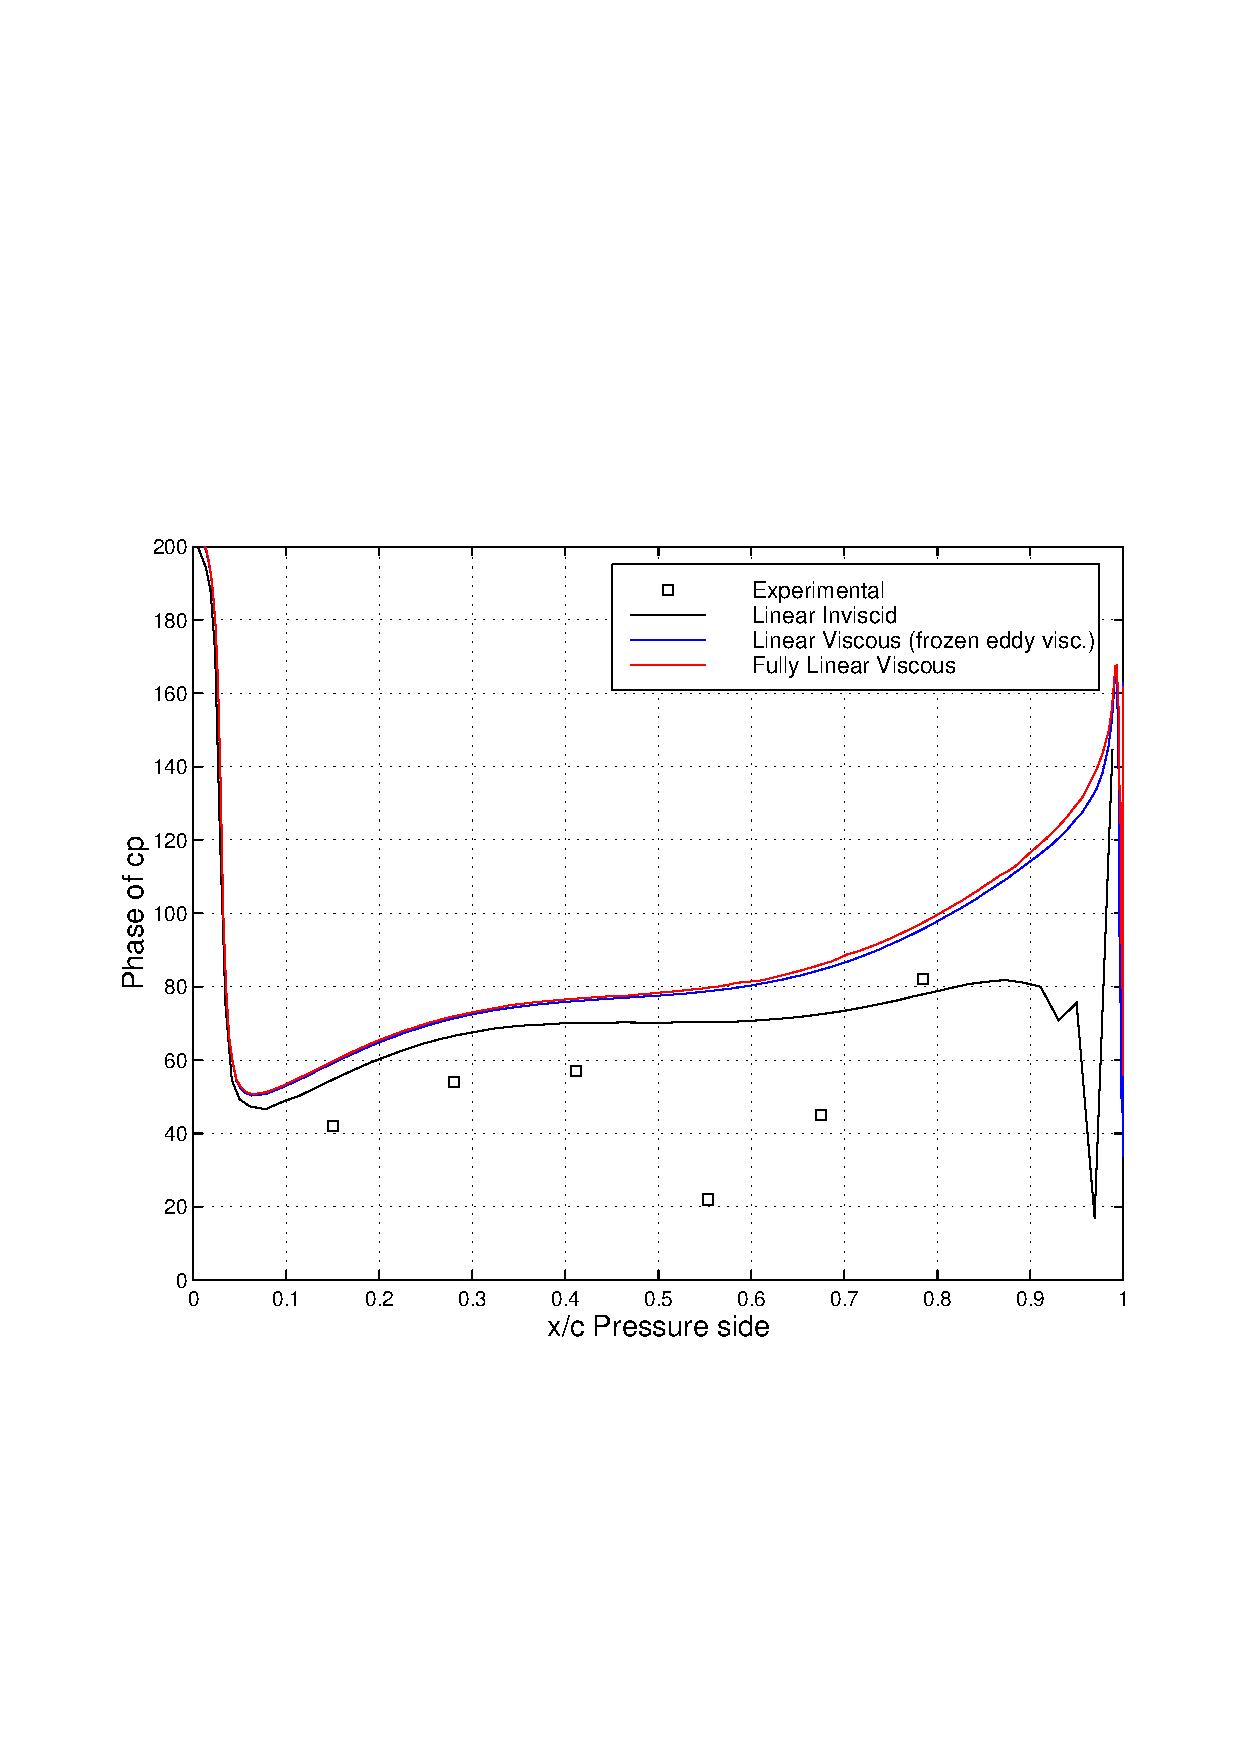
\includegraphics[height=100mm,clip=t]{CHAP_LINEAR/FIGURE/unsteady_blade_069_180_3.pdf}}\\
    {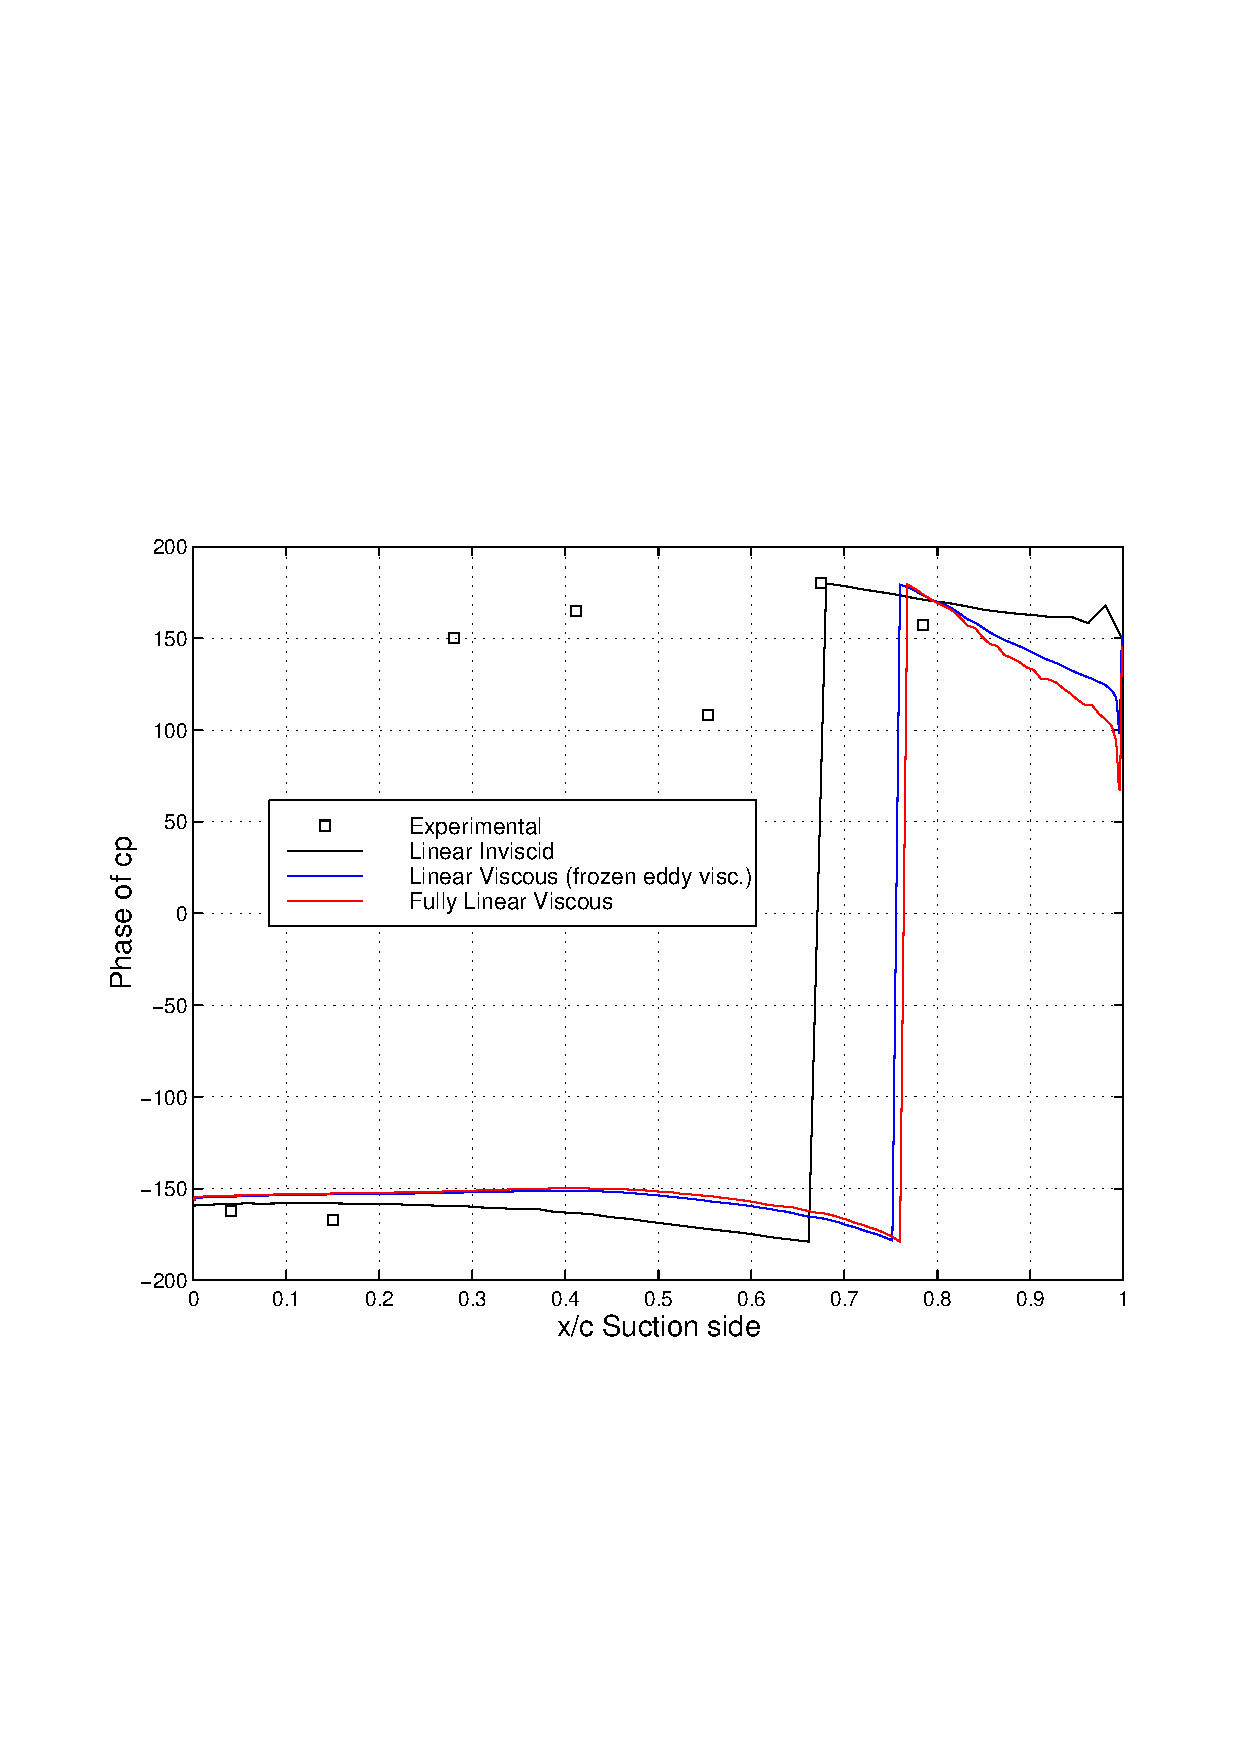
\includegraphics[height=100mm,clip=t]{CHAP_LINEAR/FIGURE/unsteady_blade_069_180_4.pdf}}
  \end{tabular}
 \end{center}
 \vspace{-7mm}
 \caption{$11^{th}$ Standard configuration - subsonic case.
          Phase of of $\tilde{c}\sm{p}$
         ($\omega = 0.21$, $\phi = 180\se{o}$)}
 \label{subsonic_11_phas.fig}
\end{figure}
%
\begin{figure}
 \begin{center}
  \begin{tabular}{c}
    {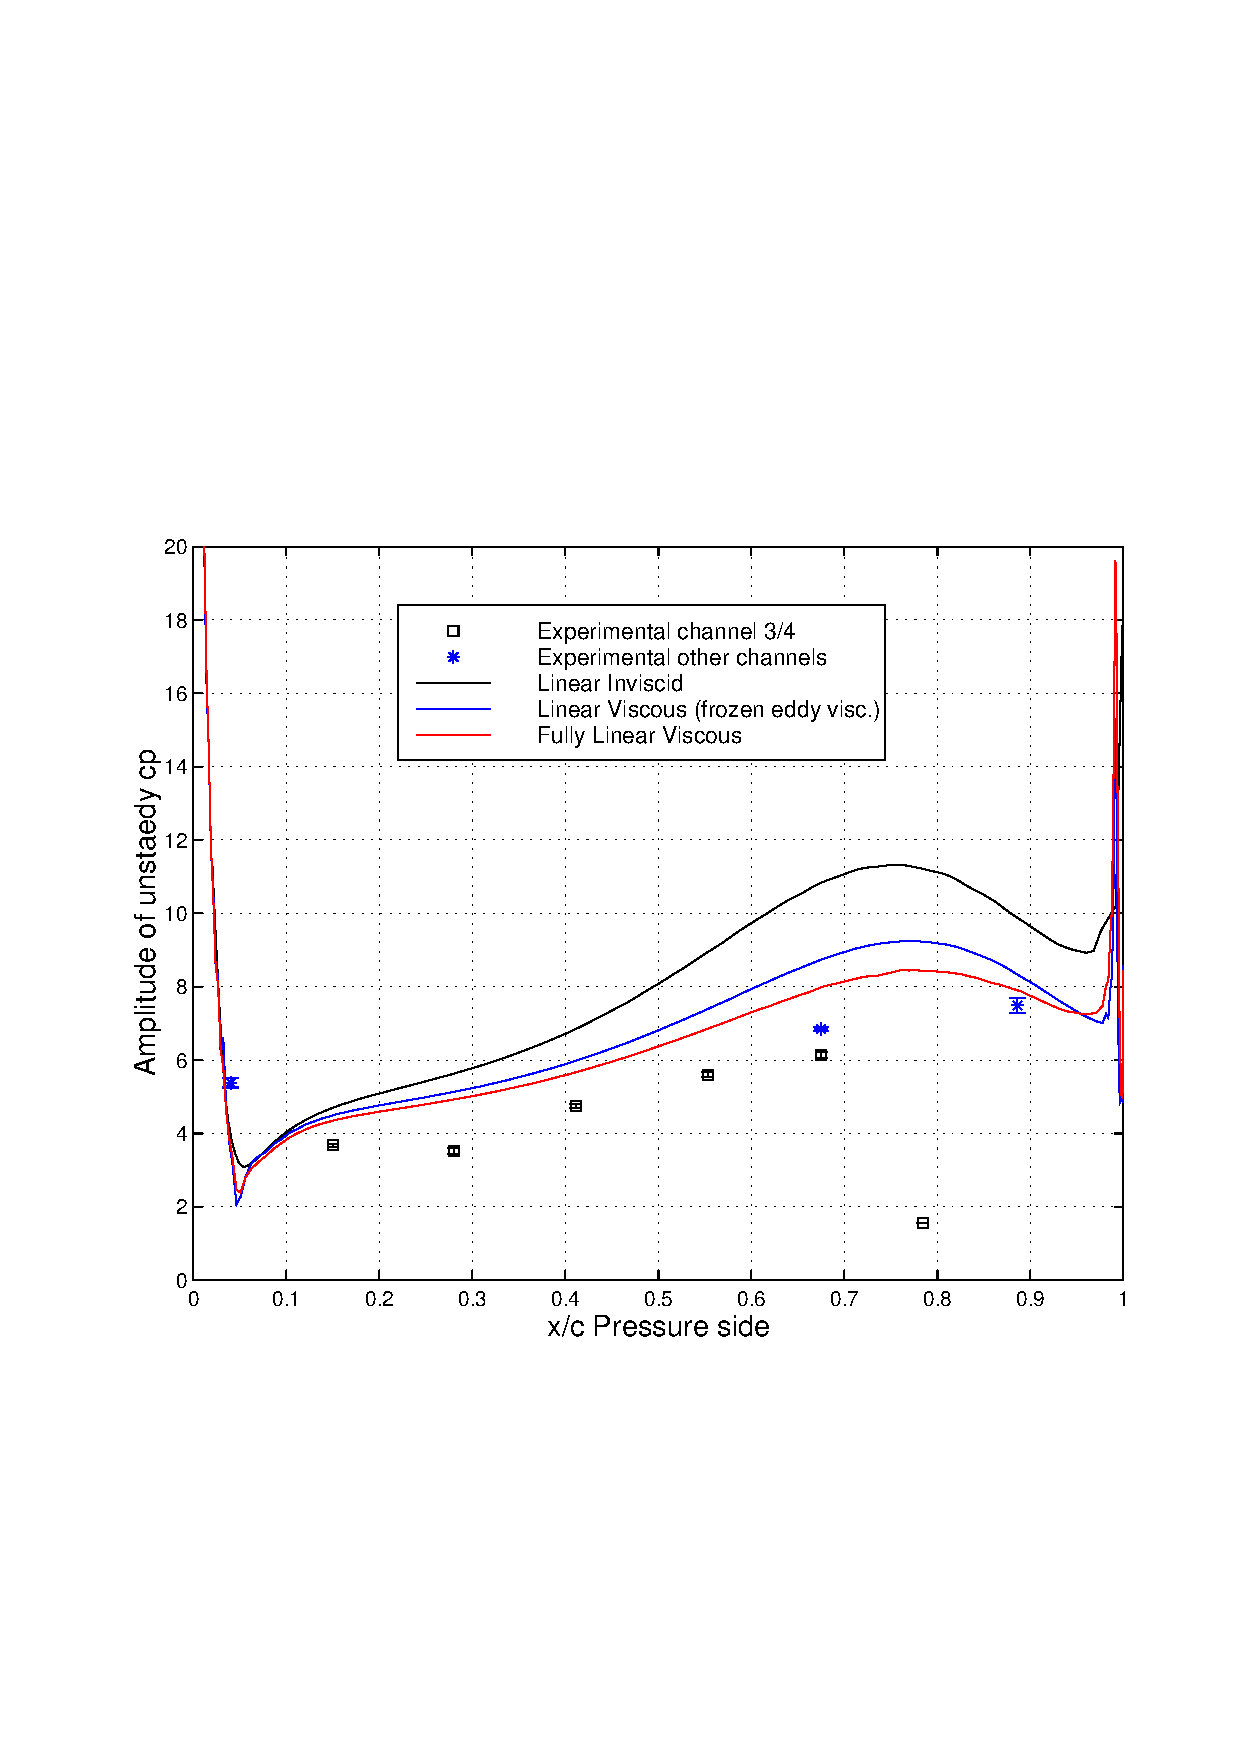
\includegraphics[height=100mm,clip=t]{CHAP_LINEAR/FIGURE/unsteady_blade_099_180_1.pdf}}\\
    {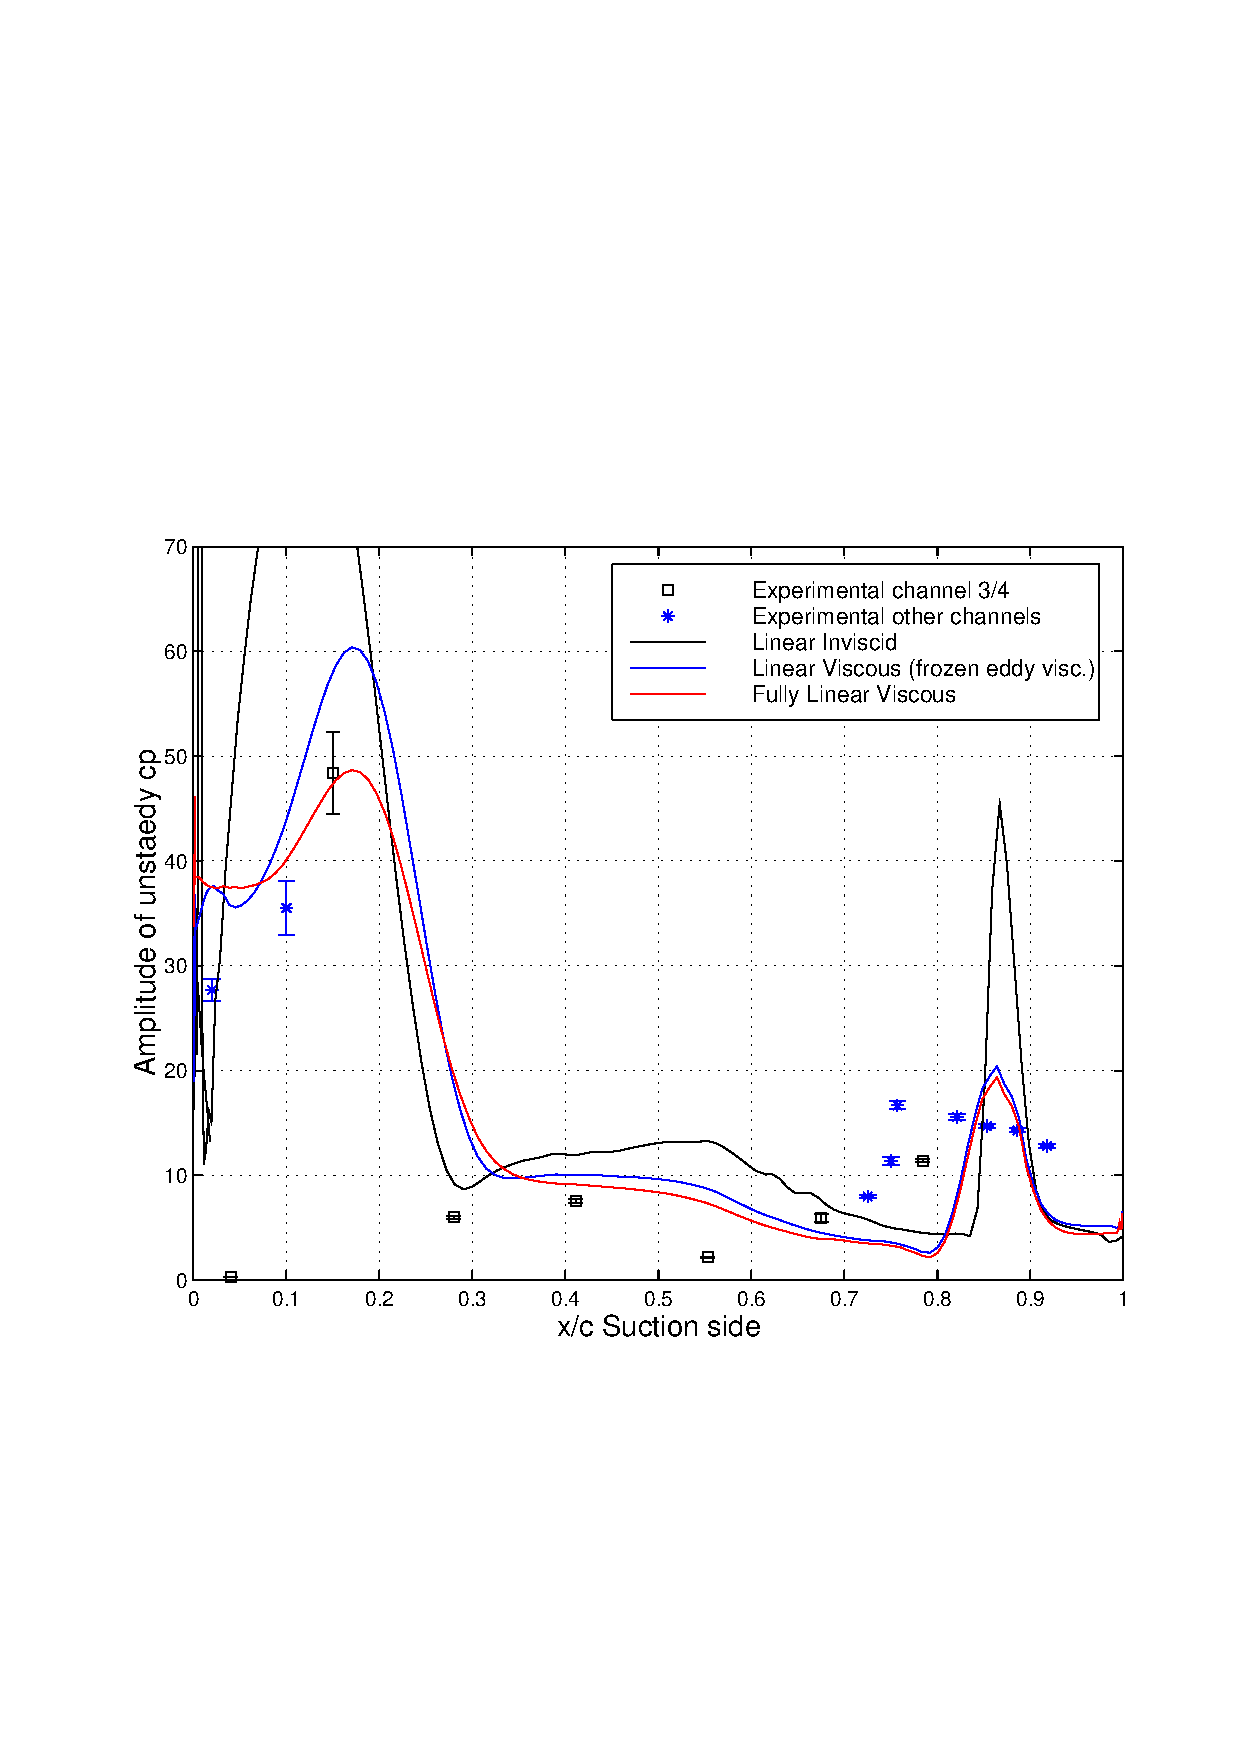
\includegraphics[height=100mm,clip=t]{CHAP_LINEAR/FIGURE/unsteady_blade_099_180_2.pdf}}
  \end{tabular}
 \end{center}
 \vspace{-7mm}
 \caption{$11^{th}$ Standard configuration - transonic case.
          Amplitude of $\tilde{c}\sm{p}$
         ($\omega = 0.15$, $\phi = 180\se{o}$)}
 \label{transonic_11_ampl.fig}
\end{figure}
%
\begin{figure}
 \begin{center}
  \begin{tabular}{c}
    {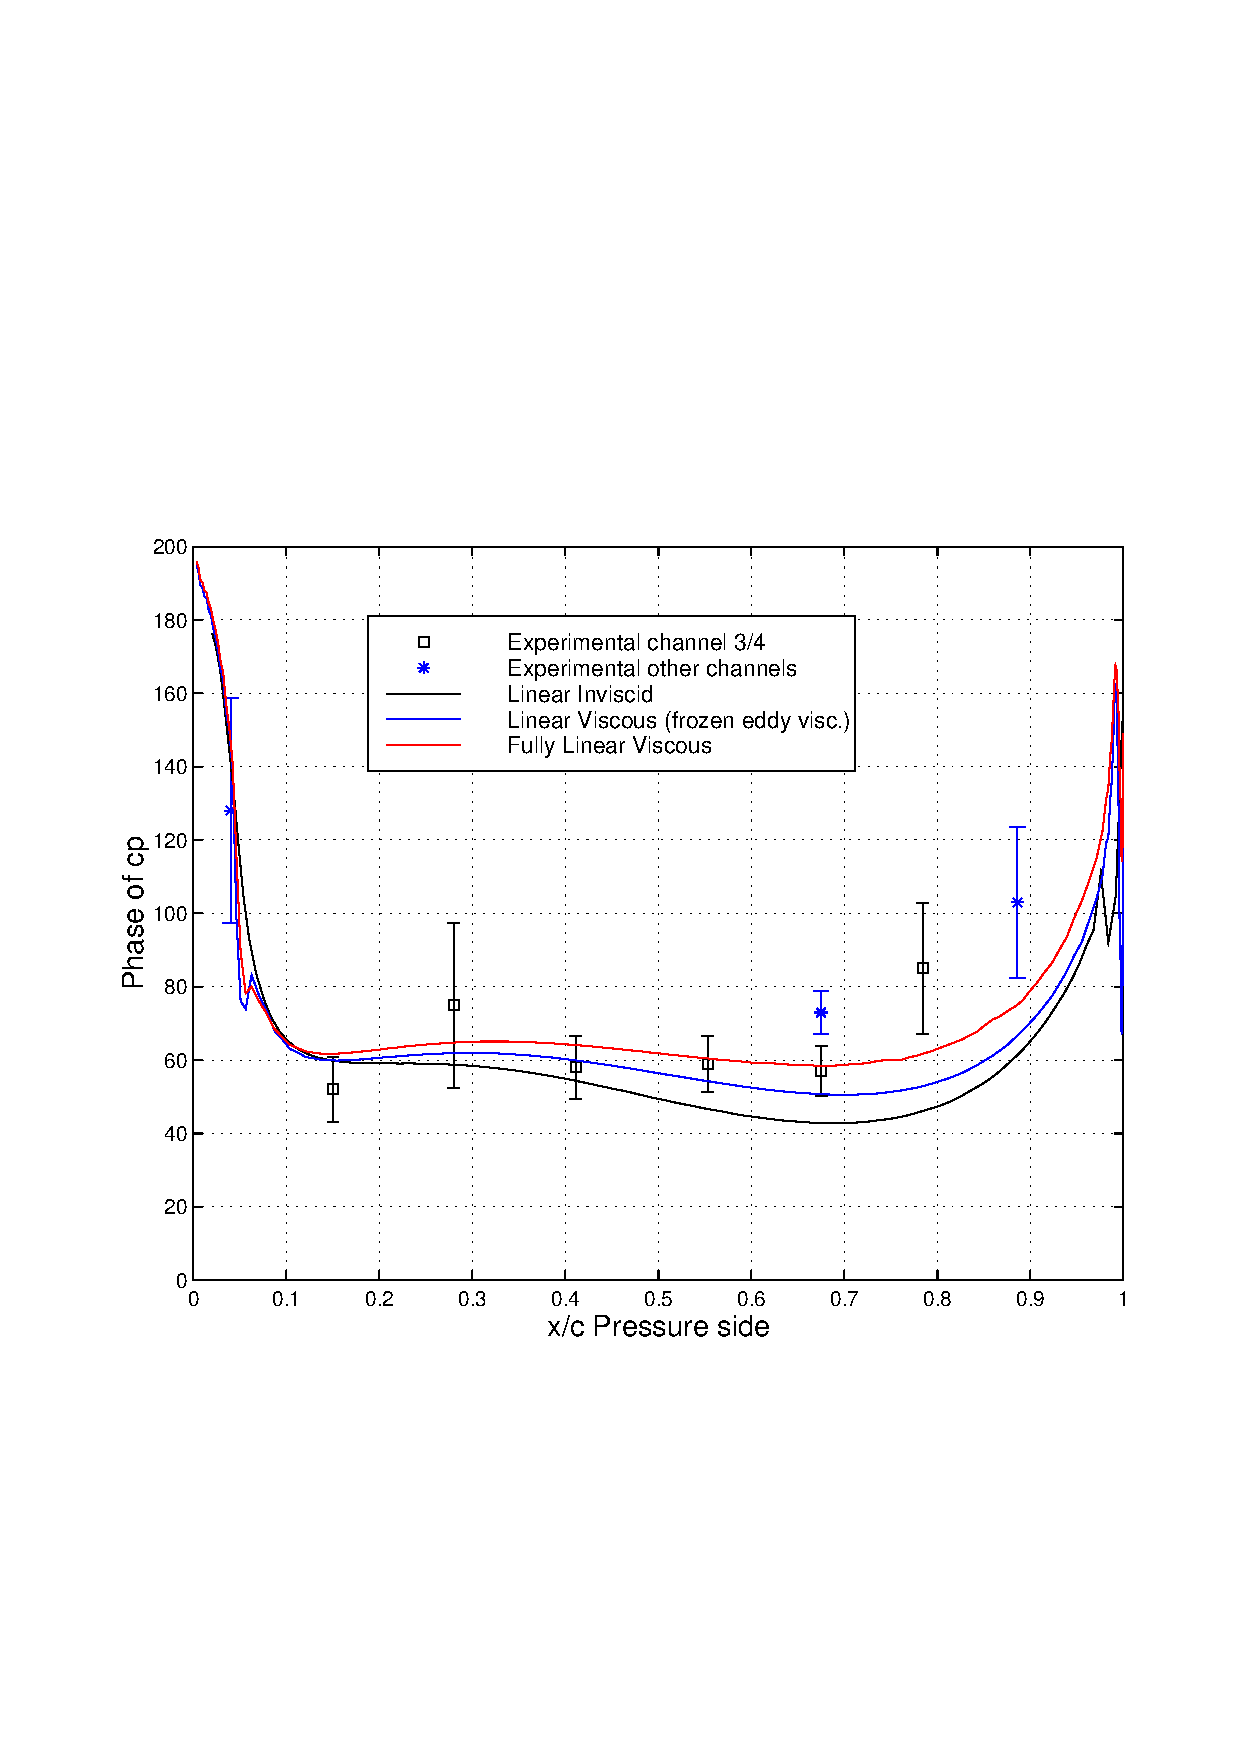
\includegraphics[height=100mm,clip=t]{CHAP_LINEAR/FIGURE/unsteady_blade_099_180_3.pdf}}\\
    {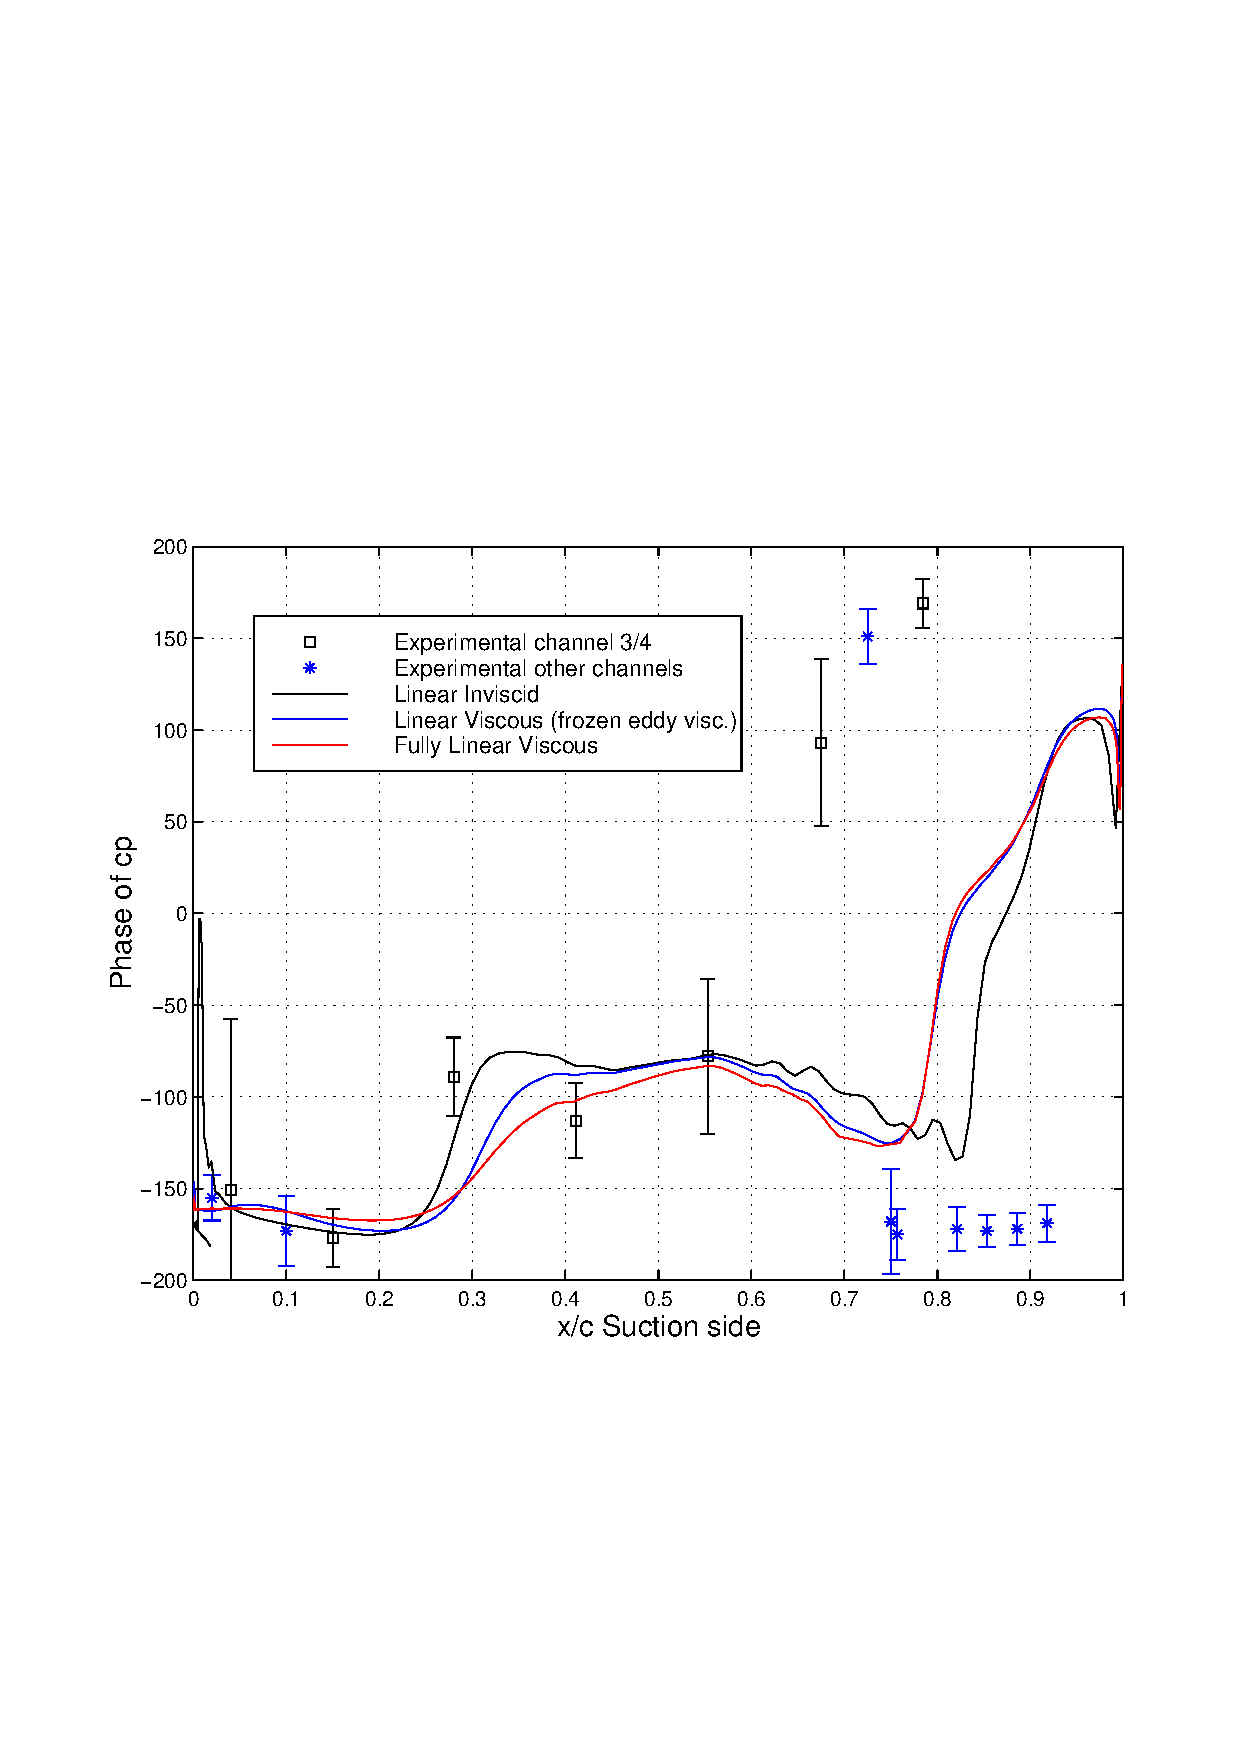
\includegraphics[height=100mm,clip=t]{CHAP_LINEAR/FIGURE/unsteady_blade_099_180_4.pdf}}
  \end{tabular}
 \end{center}
 \vspace{-7mm}
 \caption{$11^{th}$ Standard configuration - transonic case.
          Phase of of $\tilde{c}\sm{p}$
         ($\omega = 0.15$, $\phi = 180\se{o}$)}
 \label{transonic_11_phas.fig}
\end{figure}
%
